\chapter{Custom HV power supply design}

\emph{Note: the power supply design presented in this section was eventually shown not to work with the amplifier introduced in Section\,\ref{sec:hv-amplifier}. The text in this section exists to discuss why a high voltage supply is necessary, as a reference for how the experiment's power supply was built and to provide the possibility that the design be adapted in the future.}

Power op-amps don't provide significant power supply noise rejection so it is necessary to provide filtering to remove unwanted \gls{AC} components on the supply rails. As a particular supply voltage is also desired for amplifier circuits, the obvious solution is to use a \gls{DC} power supply. The most appropriate source of current for such a supply is from the mains, where the \gls{AC} sinusoidal waveform must be converted to \gls{DC}. An \gls{HV} power supply can be as simple as a mains voltage transformer (to change the peak voltage), a bridge rectifier (to remove current reversal) and filter capacitors (to suppress the sinusoidal change in voltage). This approach can be dangerous, however, due to the lack of current limit protection; and as capacitors cannot provide infinite filtering at all frequencies it leads to a compromise between having \gls{AC} components present upon the intended \gls{DC} output or dangerously high energy stored in large capacitors. Instead, a common approach is to use a power \gls{MOSFET} as a regulator. Such a circuit uses the \gls{MOSFET} as a switch to open and close the gate to keep the current flowing through it constant. As this \gls{MOSFET} operates at very high frequency (\SI{}{\mega\hertz}), the device is more than capable of removing much of the \gls{AC} component of the mains supply. Additional smoothing capacitors help to provide further filtering before and after the regulator.

Commercial \gls{HV} \gls{DC} power supplies are expensive and are typically more suited to high current applications. It was thought that the power supply for the \gls{HV} amplifier could be built from low cost components following the aforementioned \gls{MOSFET} approach, which led to the circuit shown in Figure\,\ref{fig:hv-power-supply}. The zener diodes D3-D8 set the output voltage of the positive and negative rails to be +\SI{360}{\volt} and \SI{-360}{\volt}, respectively. This design also features current limiting circuitry by means of the bipolar junction transistors T3 and T4. These use the voltage drop across \emph{witness} resistors R7 and R8 to clamp the output to the ground rail in the event of a short. If the voltage drop across R7 or R8 reaches \SI{0.7}{\volt}, corresponding to a current of \SI{70}{\milli\ampere}, each respective transistor opens up a low resistance path to ground for the field normally facilitating current flow through the \gls{MOSFET}, effectively halting the output current.

The addition of \glspl{LED} (D11 and D12) allows for visual identification of current output. Each \gls{LED}'s brightness is proportional to the current flow, giving an indication of whether the output is live. In the event that the overcurrent protection is tripped, these \glspl{LED} will extinguish.

\begin{figure}
  \centering
  \includegraphics[width=\columnwidth]{graphics/generated/from-svg/60-hv-power-supply.pdf}
  \caption{\gls{HV} power supply design. This circuit uses a transformer, bridge rectifier, \gls{MOSFET} regulator, zener diodes and smoothing capacitors. It is an evolution on a single-sided power supply by Henning Valbruch (AEI, Hannover), following the \emph{de-facto} standard design \cite{Horowitz2015}, with the addition of a negative output rail and current limiting circuitry. This design \emph{does not} work with the \gls{HV} amplifier as discussed in Section\,\ref{sec:hv-amplifier}\textemdash see Section\,\ref{sec:hv-psu-amp-measurements} for more details.}
  \label{fig:hv-power-supply}
\end{figure}

The power dissipated in each \gls{MOSFET} in certain circumstances can reach \SI{50}{\watt}, so sufficient heat sinks are required. For this design the choice was made to mount L-shaped angle brackets to the enclosure and the circuit board, onto which the \gls{MOSFET} casings were fixed. These brackets were further connected via the enclosure to large metal fins. \note{Photo?}
% 50W claim: see Ken's email, 2016-01-19 11:56. Device can withstand 100mA @ 500V for brief periods.